\documentclass[french]{book}
\usepackage[utf8]{inputenc}
\usepackage[french]{babel}
%\usepackage{teach}
\usepackage{verbatim}
\usepackage{amsmath,amsfonts,amssymb}
\usepackage{pgf,pgfplots,tikz,tkz-tab}
\usepackage{mathrsfs}
\usepackage{multicol}
\usepackage{lscape}
\usepackage{pstricks-add}
%\pgfplotsset{compat=1.15}
\usetikzlibrary{arrows}
%\redefinecolor{thm}{title}{bgcolor}{alizarin}
%\redefinecolor{prop}{title}{bgcolor}{meatbrown}
%\redefinecolor{defn}{title}{bgcolor}{olivine}
\definecolor{alizarin}{rgb}{0.82, 0.1, 0.26}
\definecolor{meatbrown}{rgb}{0.9, 0.72, 0.23}
\definecolor{olivine}{rgb}{0.6, 0.73, 0.45}
\usepackage{geometry}
%\geometry{top=1cm, bottom=1cm, left=2cm, right=2cm}
\geometry{hmargin=1cm,vmargin=0.5cm}
\pagestyle{empty}
\begin{document}
\section*{Devoir surveillé I}
\subsection*{Exercice 1 - La fonction "cloche"}
Voici une représentation graphique d'une partie de fonction $f$ bien connue appelée fonction aussi "cloche".

\begin{center}
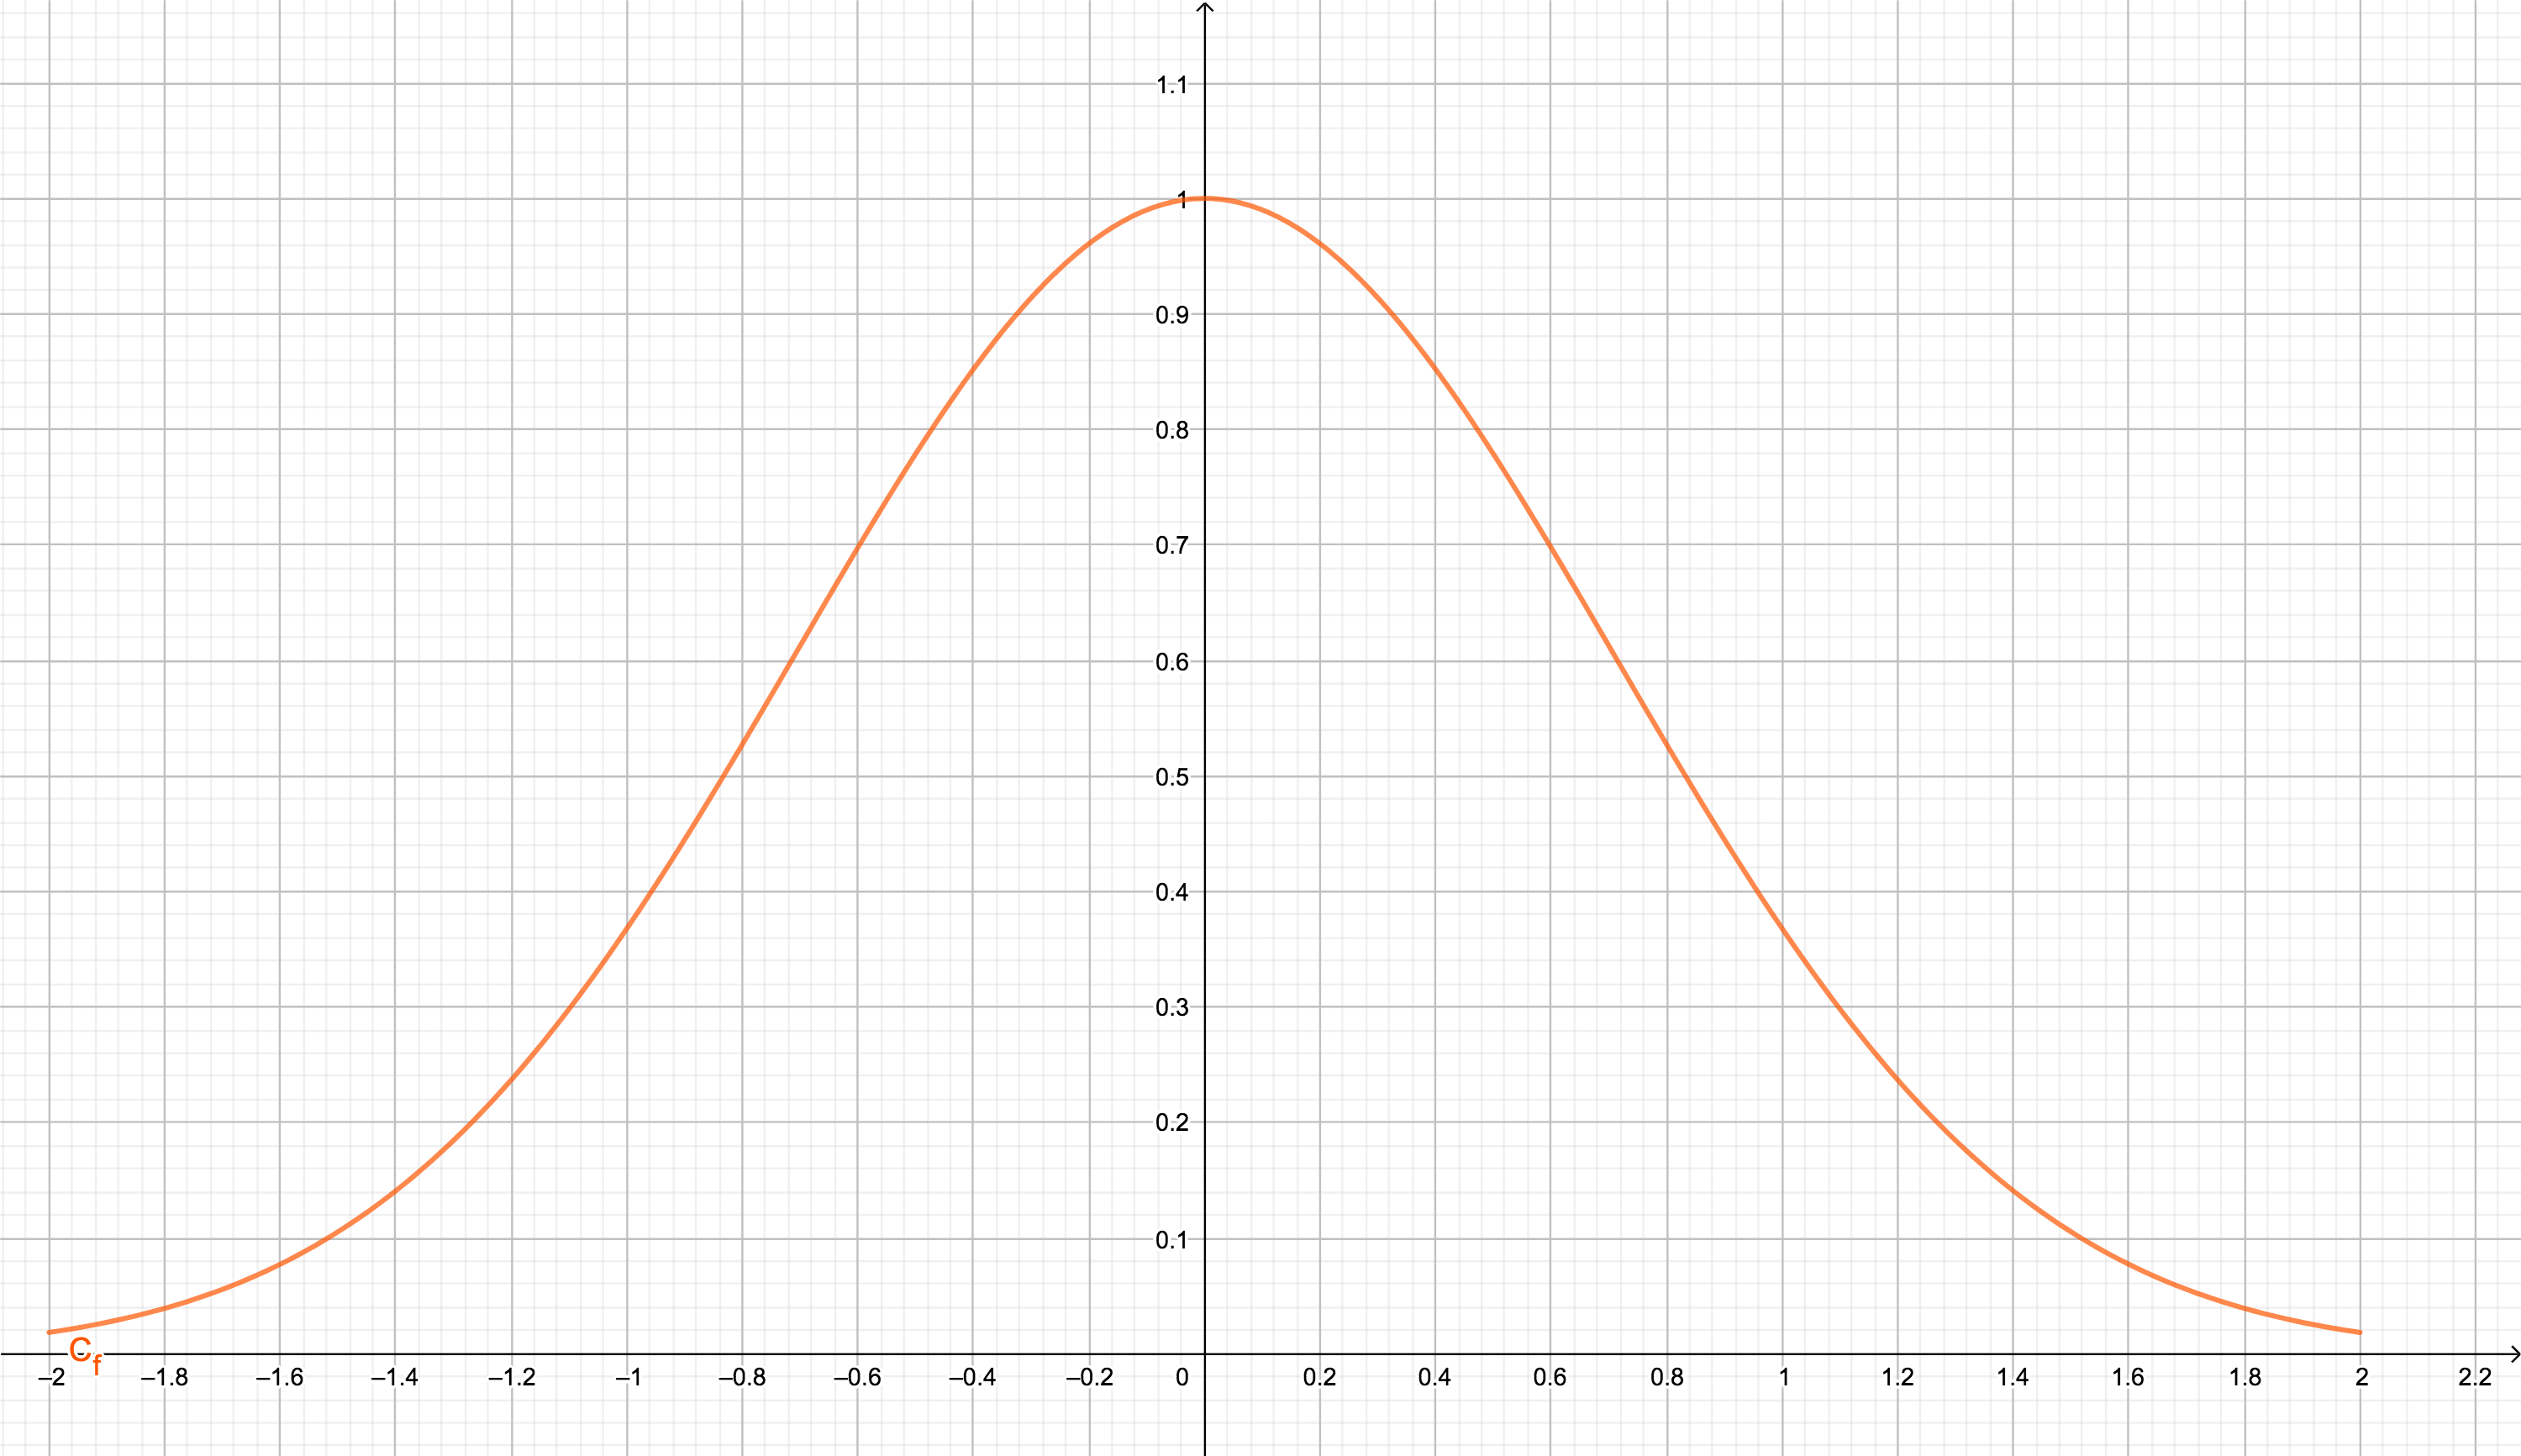
\includegraphics[scale=4]{monimage2.png} 
\end{center}



\begin{itemize}
\item[A)]Quel est l'ensemble de définition de la fonction ? 
\item[B)]Déterminer graphiquement l'image de $0;1;2;-1;-2$.
\item[C)]Déterminer graphiquement, s'il(s) existe(nt), tous les antécédants de $1;0$ et $0,5$ par la fonction $f$, préciser si celui-çi est unique quand c'est le cas.
\item[D)]Pouvez vous dire si la fonction est paire, impaire ou aucun des deux ?
\item[E)]Faire le tableau de variation de $f$.
\item[F)]Résoudre $f(x) \geq 0,5$.

\end{itemize} 


\subsection*{Exercice 2 - Multiples et diviseurs}
Recopier les phrases suivantes en complétant par "multiple" ou "diviseur":

\begin{itemize}
\item[A)]2500 est un ... de 500.

\item[B)]1 est un ... de 1000.

\item[C)]30 est un ... de 0.

\item[D)]2 est un ... de 56.

\item[E)]3 est un ... de $111 \, 111 \, 111 \, 111$.

\item[F)]10 est un ... de 10.
\end{itemize}

\subsection*{Exercice 3 - Harmonique et musique}
Si on appelle $f$ la fréquence fondamentale, les partiels harmoniques ont des fréquences égales à : 2$f$, 3$f$, 4$f$, 5$f$, etc.\\

Recopier les deux phrases suivantes en complétant par "multiple" ou "diviseur":

\begin{itemize}
\item[A)]les partiels harmoniques sont des ... de la fréquence fondamentale.
\item[B)]la fréquence fondamentale est un ... des partiels harmoniques.
\item[C)]En prenant comme note fondamentale $la_3$ du piano ayant pour fréquence fondamentale de 440 Hz, donner les trois premiers partiels harmoniques de $la_3$.
\item[D)]Est-il possible qu'un partiels harmoniques d'une certaine note soit un nombre premier? Justifiez soigneusement votre réponse de manière concise.
\end{itemize} 

\newpage
\subsection*{Exercice 4 - Irréductibilité de fraction}
Simplifier au maximum quand cela est possible:
$$ \frac{3}{7}; \;  \frac{9}{49}; \;  \frac{57}{3}; \;  \frac{100}{2}; \;  \frac{9}{2}; \;  \frac{48}{4}. $$

\subsection*{Exercice 5 - Un grand nombre}

Décomposer en produit de nombre premier le nombre suivant: $6 \; 630$.


 \end{document}


\subsection*{Exercice 5 - Diviseur de tension}

Suite à un problème électrique, la seule prise de votre chambre délivre 440 volts au lieu de 220 volts habituel, pour remédier à ce problème rapidement, vous décidez de faire appel à un montage électrique: le diviseur de tension.

%inserer image
\begin{center}
\includegraphics[scale=0.5]{monimage.png} 
\end{center}


 C'est un montage "simple" qui permet de diviser une tension d'entrée $U$ et de délivrer une tension de sortie $U_2$ plus petite que $U$.

Pour cela on a besoin de deux résistances que l'on note $R_1,R_2$, la tension de sortie $U_2$ est donnée pas l'égalité suivante:
$$U_2=U.\frac{R_1}{R_1+R_2}$$ 

\begin{itemize}
\item[A)]En sachant ici que $U=440$ et $U_2=220$ et $R_2=1$ déterminer la valeur de $R_1$.\\

\end{itemize}
Maintenant que le diviseur de tension est fonctionnel, on dispose au final de deux tensions de sortie $U_2$ que l'on connait déjà et $U_1$ qui à pour valeur: 
$$U_1=U.\frac{R_2}{R_1+R_2}$$ 


\begin{itemize}
\item[B)]Calculer $U_1$, que remarque t-on avec $U_2$? Est-ce toujours le cas? Donner un contre-exemple si cela est faux.
\item[C)] On suppose pour finir que $R_2=1$, $U=101$ qui est un nombre premier et que $U_2 \in \mathbb{N}$, déterminer $R_1$. 
\end{itemize}